\section{圆周的基本群}
\label{section:ch09-sec54}

空间 $X$ 的覆叠空间的研究与 $X$ 的基本群的研究是密切相关的. 在本节中我们将建立这两个概念之间的几个重要的联系, 并且计算圆周的基本群.

\begin{definition}[提升]
\label{definition:ch09-sec54-lifting}
设 $p\colon E\to B$ 是一个映射. 如果 $f$ 是从某一空间 $X$ 到 $B$ 中的一个连续映射, 映射 $\tilde{f}\colon X\to E$ 若满足条件 $p\circ\tilde{f}=f$, 即有下述图表可交换, 则称 $\tilde{f}$ 为 $f$ 的一个\textbf{提升}(lifting).
\[
\begin{array}{ccc}
 & E & \\
\tilde{f}\nearrow & \downarrow p & \\
X & \longrightarrow & B \\
 & f &
\end{array}
\]
\end{definition}

当 $p$ 是覆叠映射时, 提升的存在性对于研究覆叠空间以及基本群都十分重要. 首先我们证明对于一个覆叠空间, 道路能够提升, 然后证明道路同伦也能提升. 先给出一个例子.

\begin{example}
\label{example:ch09-sec54-1}
考虑定理 \cref{theorem:ch09-sec53-53-1} 中的覆叠映射 $p\colon\mathbb{R}\to S^{1}$. 以 $b_0=(1,0)$ 为起点、定义为 $f(s)=(\cos\pi s,\sin\pi s)$ 的道路 $f$, 提升为以 $0$ 为起点、以 $\frac{1}{2}$ 为终点的道路 $\tilde{f}(s)=s/2$. 道路 $g(s)=(\cos\pi s,-\sin\pi s)$ 提升为以 $0$ 为起点、以 $-\frac{1}{2}$ 为终点的道路 $\tilde{g}(s)=-s/2$. 道路 $h(s)=(\cos 4\pi s,\sin 4\pi s)$ 提升为以 $0$ 为起点、以 $2$ 为终点的道路 $\tilde{h}(s)=2s$. 直观地说, $h$ 将区间 $[0,1]$ 绕着圆周转两圈, 这一点反映在提升道路 $\tilde{h}$ 从 $0$ 开始到 $2$ 结束这一事实中. 这些道路都画在图 \cref{figure:ch09-fig-54-1} 中.
\end{example}

\par
\begin{figure}[htbp]
\centering
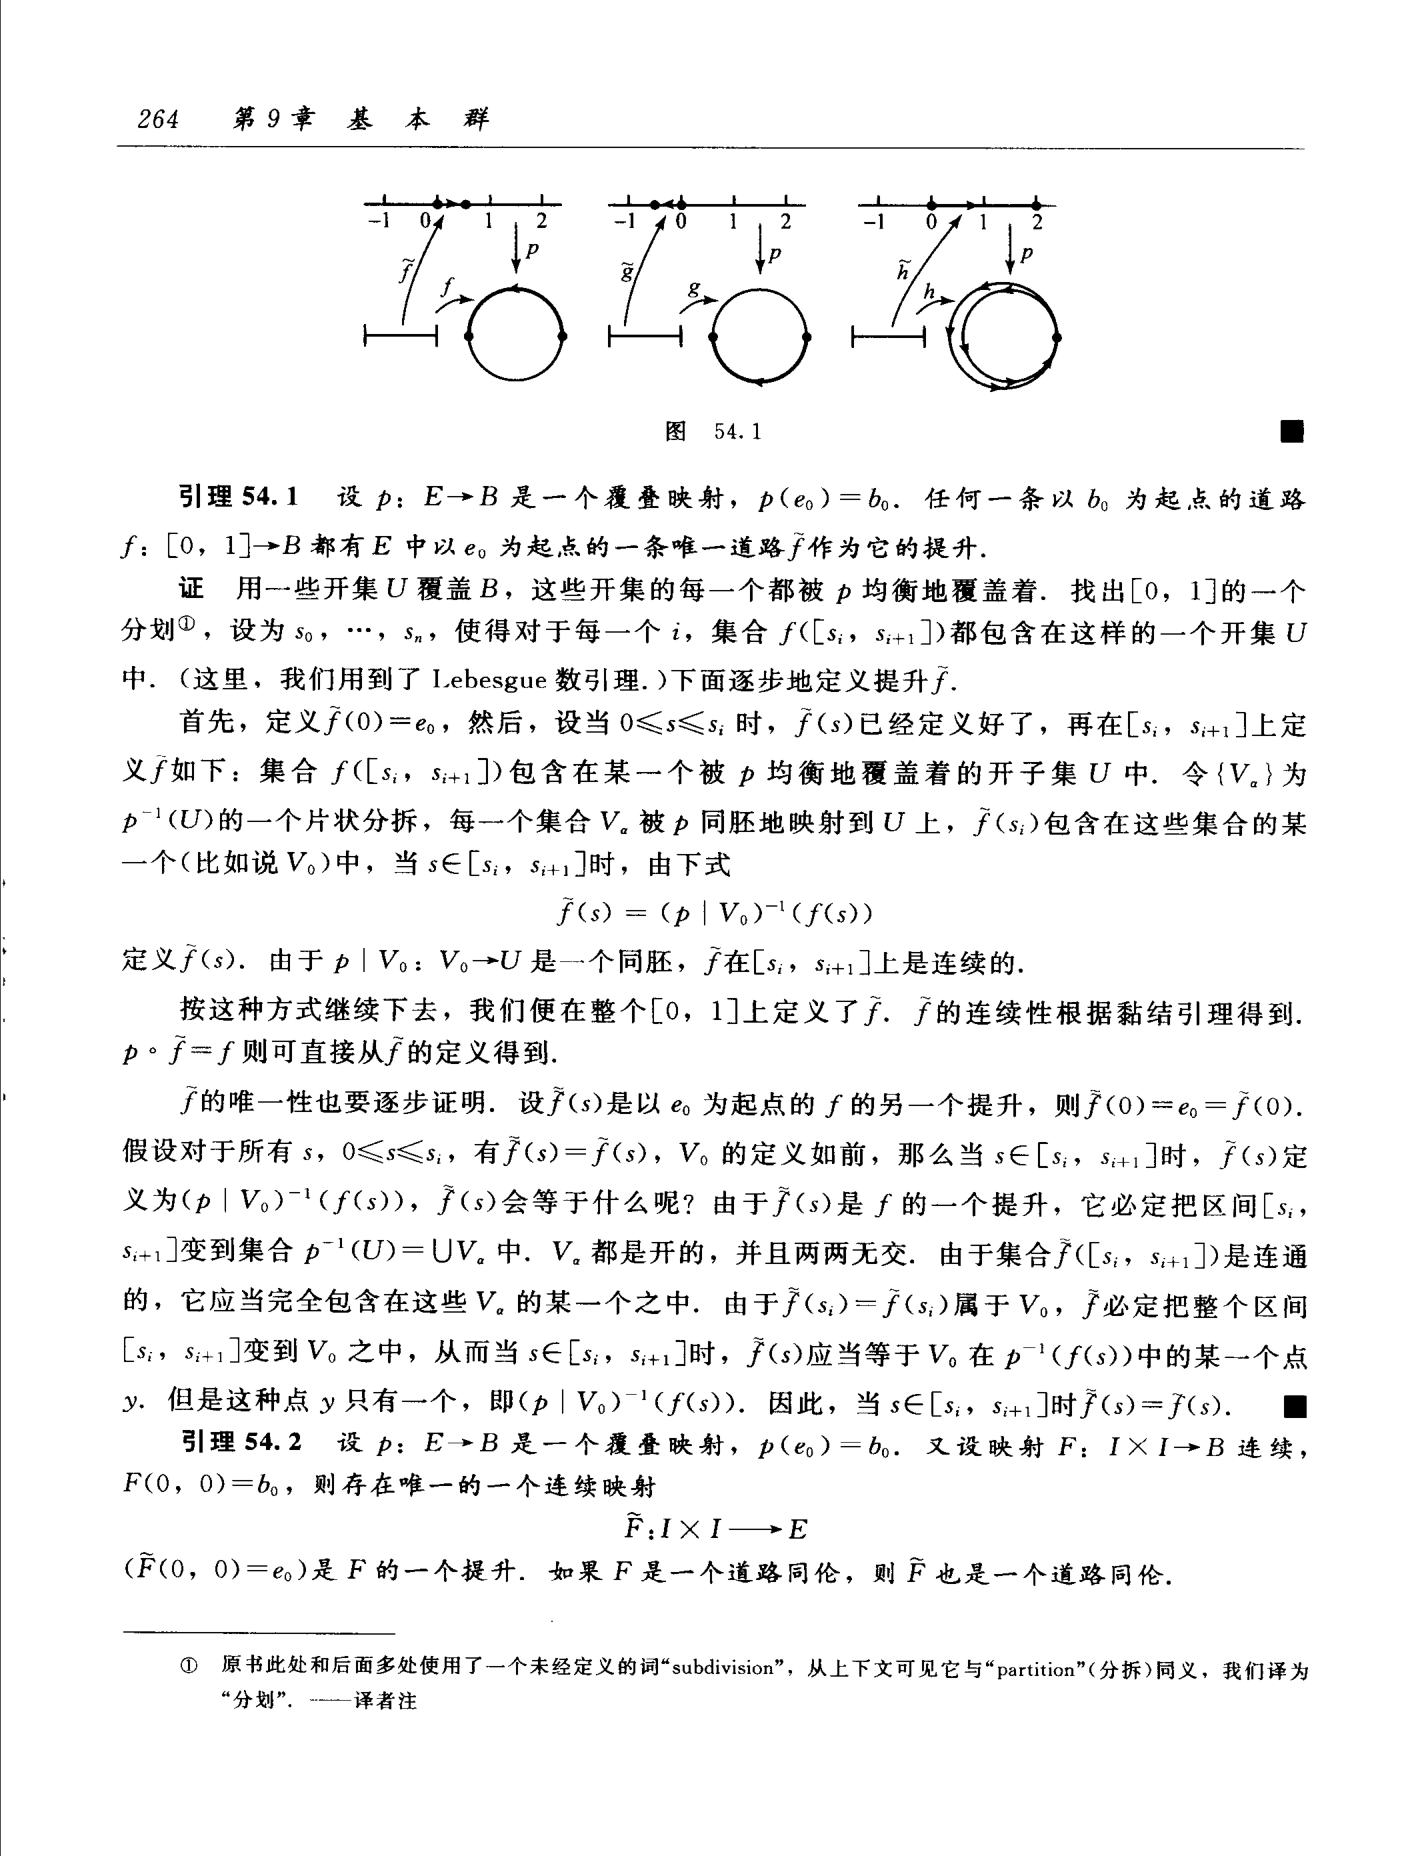
\includegraphics[width=0.7\textwidth]{image/fig-54-1.png}
\caption{道路的提升.}
\label{figure:ch09-fig-54-1}
\end{figure}

\begin{lemma}[道路提升引理]
\label{lemma:ch09-sec54-54-1}
设 $p\colon E\to B$ 是一个覆叠映射, $p(e_0)=b_0$. 任何一条以 $b_0$ 为起点的道路 $f\colon[0,1]\to B$ 都有 $E$ 中以 $e_0$ 为起点的一条唯一道路 $\tilde{f}$ 作为它的提升.
\end{lemma}

\begin{proof}
用一些开集 $U$ 覆盖 $B$, 这些开集的每一个都被 $p$ 均衡地覆盖着. 找出 $[0,1]$ 的一个分划, 设为 $s_0,\cdots,s_n$, 使得对于每一个 $i$, 集合 $f([s_i,s_{i+1}])$ 都包含在这样的一个开集 $U$ 中. (这里用到了 Lebesgue 数引理.) 下面逐步地定义提升 $\tilde{f}$.

首先, 定义 $\tilde{f}(0)=e_0$, 然后, 设当 $0\leqslant s\leqslant s_i$ 时, $\tilde{f}(s)$ 已经定义好了, 再在 $[s_i,s_{i+1}]$ 上定义 $\tilde{f}$ 如下: 集合 $f([s_i,s_{i+1}])$ 包含在某一个被 $p$ 均衡地覆盖着的开子集 $U$ 中. 令 $\{V_\alpha\}$ 为 $p^{-1}(U)$ 的一个片状分拆, 每一个集合 $V_\alpha$ 被 $p$ 同胚地映射到 $U$ 上, $\tilde{f}(s_i)$ 包含在这些集合的某一个 (比如说 $V_0$) 中, 当 $s\in[s_i,s_{i+1}]$ 时, 由下式
\[
\tilde{f}(s)=(p\mid V_{0})^{-1}(f(s))
\]
定义 $\tilde{f}(s)$. 由于 $p\mid V_0\colon V_0\to U$ 是一个同胚, $\tilde{f}$ 在 $[s_i,s_{i+1}]$ 上是连续的.

按这种方式继续下去, 我们便在整个 $[0,1]$ 上定义了 $\tilde{f}$. $\tilde{f}$ 的连续性根据黏结引理得到. $p\circ\tilde{f}=f$ 则可直接从 $\tilde{f}$ 的定义得到.

$\tilde{f}$ 的唯一性也要逐步证明. 设 $\tilde{f}'(s)$ 是以 $e_0$ 为起点的 $f$ 的另一个提升, 则 $\tilde{f}'(0)=e_0=\tilde{f}(0)$. 假设对于所有 $s$, $0\leqslant s\leqslant s_i$, 有 $\tilde{f}'(s)=\tilde{f}(s)$, $V_0$ 的定义如前, 那么当 $s\in[s_i,s_{i+1}]$ 时, $\tilde{f}'(s)$ 定义为 $(p\mid V_0)^{-1}(f(s))$, $\tilde{f}(s)$ 会等于什么呢? 由于 $\tilde{f}'(s)$ 是 $f$ 的一个提升, 它必定把区间 $[s_i,s_{i+1}]$ 变到集合 $p^{-1}(U)=\bigcup V_\alpha$ 中. $V_\alpha$ 都是开的, 并且两两无交. 由于集合 $\tilde{f}'([s_i,s_{i+1}])$ 是连通的, 它应当完全包含在这些 $V_\alpha$ 的某一个之中. 由于 $\tilde{f}'(s_i)=\tilde{f}(s_i)$ 属于 $V_0$, $\tilde{f}'$ 必定把整个区间 $[s_i,s_{i+1}]$ 变到 $V_0$ 之中, 从而当 $s\in[s_i,s_{i+1}]$ 时, $\tilde{f}'(s)$ 应当等于 $V_0$ 在 $p^{-1}(f(s))$ 中的某一个点 $y$. 但是这种点 $y$ 只有一个, 即 $(p\mid V_0)^{-1}(f(s))$. 因此, 当 $s\in[s_i,s_{i+1}]$ 时 $\tilde{f}'(s)=\tilde{f}(s)$.
\end{proof}

\begin{lemma}[同伦提升引理]
\label{lemma:ch09-sec54-54-2}
设 $p\colon E\to B$ 是一个覆叠映射, $p(e_0)=b_0$. 又设映射 $F\colon I\times I\to B$ 连续, $F(0,0)=b_0$, 则存在唯一的一个连续映射
\[
\widetilde{F}\colon I\times I\longrightarrow E
\]
$(\widetilde{F}(0,0)=e_0)$ 是 $F$ 的一个提升. 如果 $F$ 是一个道路同伦, 则 $\widetilde{F}$ 也是一个道路同伦.
\end{lemma}

\par
\begin{figure}[htbp]
\centering
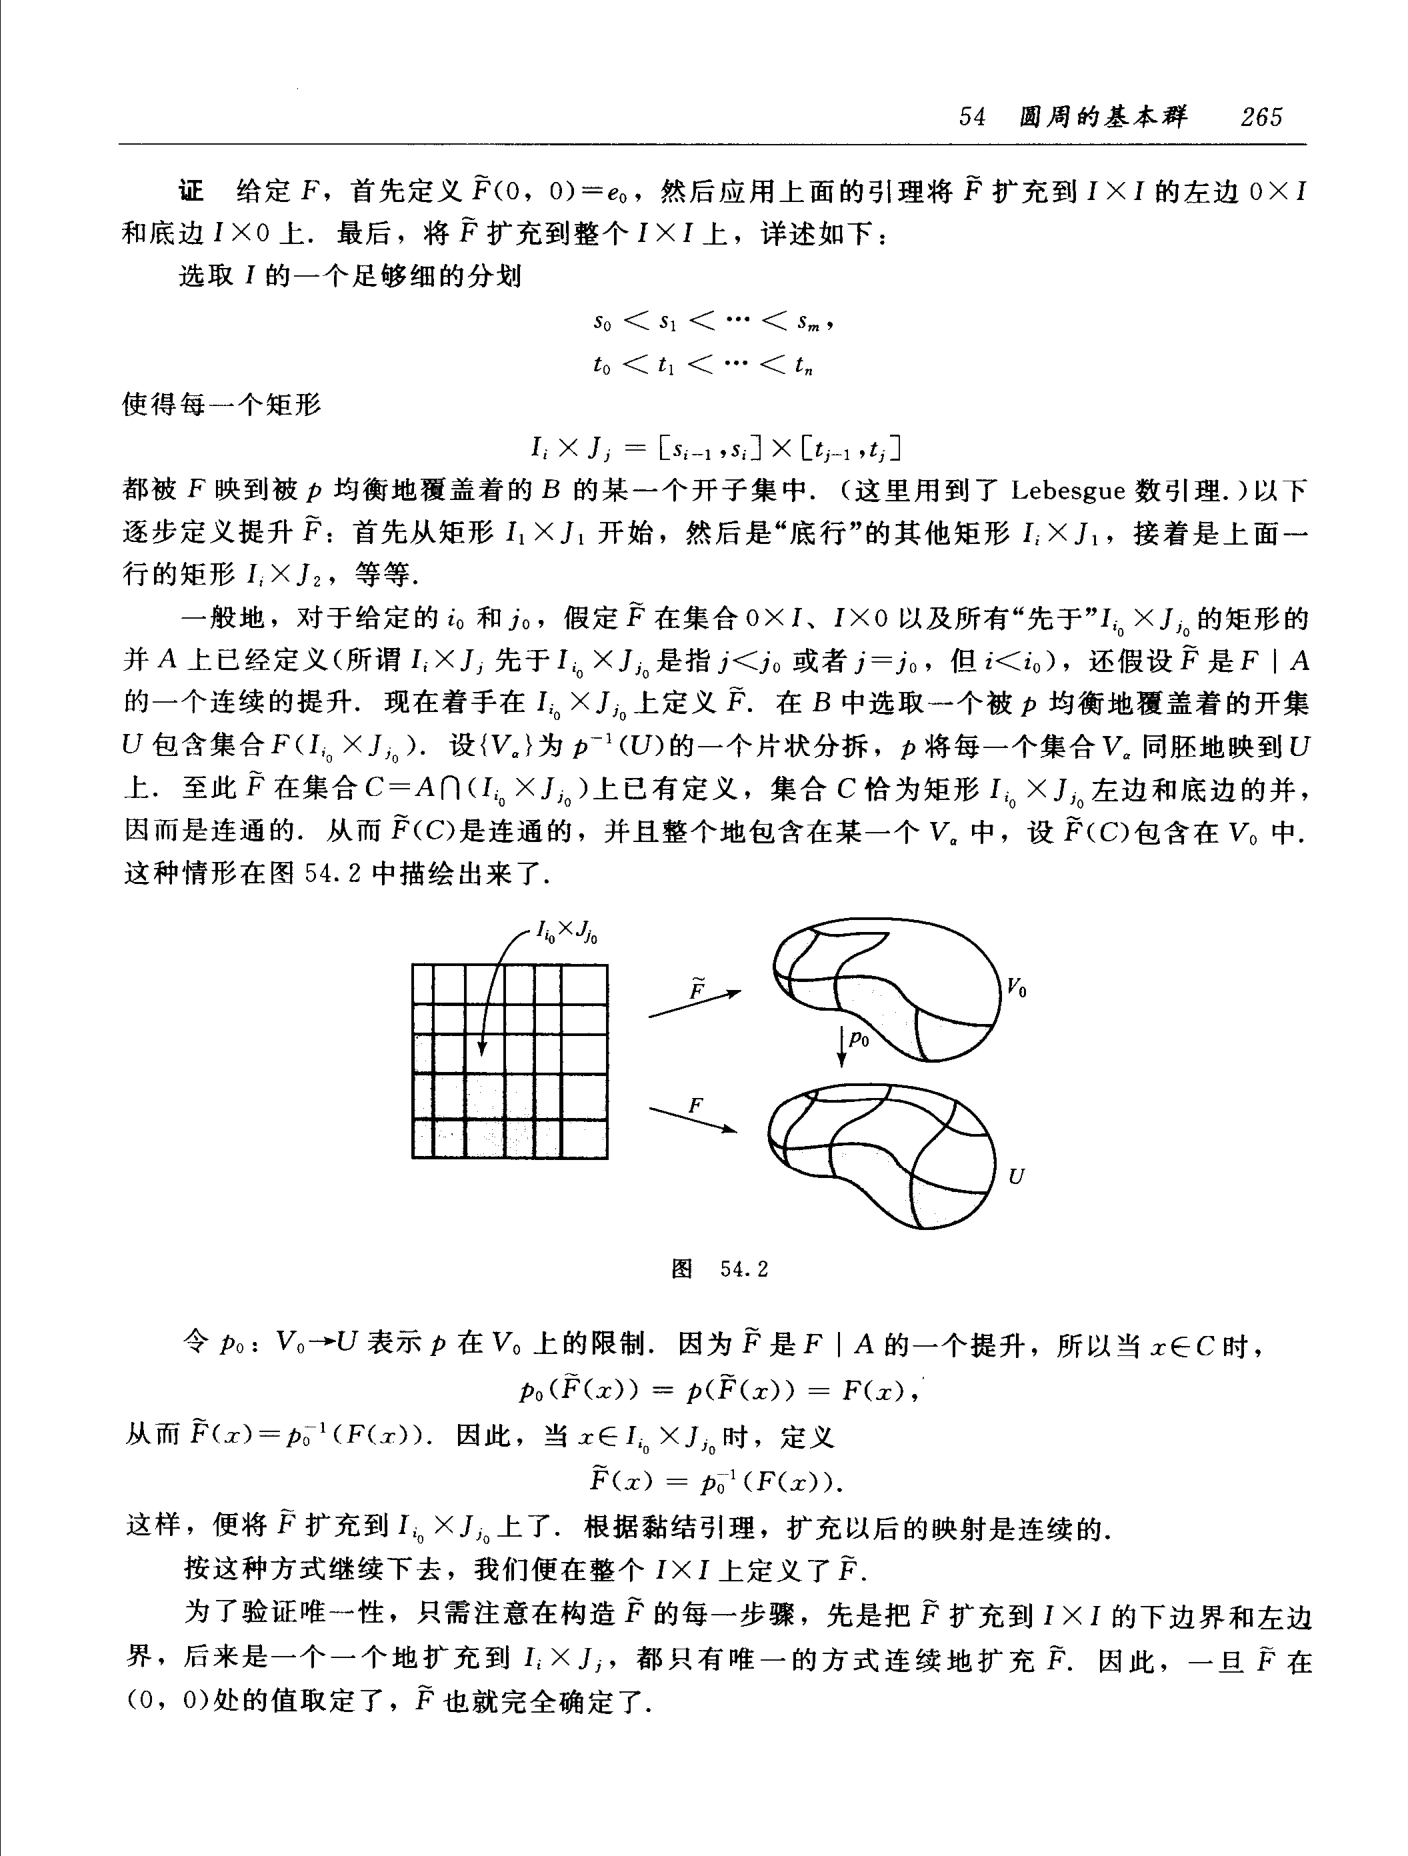
\includegraphics[width=0.7\textwidth]{image/fig-54-2.png}
\caption{同伦提升.}
\label{figure:ch09-fig-54-2}
\end{figure}

\begin{proof}
给定 $F$, 首先定义 $\widetilde{F}(0,0)=e_0$, 然后应用上面的引理将 $\widetilde{F}$ 扩充到 $I\times I$ 的左边 $0\times I$ 和底边 $I\times 0$ 上. 最后, 将 $\widetilde{F}$ 扩充到整个 $I\times I$ 上, 详述如下:

选取 $I$ 的一个足够细的分划
\[
s_{0}<s_{1}<\cdots<s_{m},\qquad
t_{0}<t_{1}<\cdots<t_{n},
\]
使得每一个矩形
\[
I_{i}\times J_{j}=[s_{i-1},s_{i}]\times[t_{j-1},t_{j}]
\]
都被 $F$ 映到被 $p$ 均衡地覆盖着的 $B$ 的某一个开子集中. (这里用到了 Lebesgue 数引理.) 以下逐步定义提升 $\widetilde{F}$: 首先从矩形 $I_1\times J_1$ 开始, 然后是"底行"的其他矩形 $I_i\times J_1$, 接着是上面一行的矩形 $I_i\times J_2$, 等等.

一般地, 对于给定的 $i_0$ 和 $j_0$, 假定 $\widetilde{F}$ 在集合 $0\times I$、$I\times 0$ 以及所有"先于" $I_{i_0}\times J_{j_0}$ 的矩形的并 $A$ 上已经定义 (所谓 $I_i\times J_j$ 先于 $I_{i_0}\times J_{j_0}$ 是指 $j<j_0$ 或者 $j=j_0$, 但 $i<i_0$), 还假设 $\widetilde{F}$ 是 $F\mid A$ 的一个连续的提升. 现在着手在 $I_{i_0}\times J_{j_0}$ 上定义 $\widetilde{F}$. 在 $B$ 中选取一个被 $p$ 均衡地覆盖着的开集 $U$ 包含集合 $F(I_{i_0}\times J_{j_0})$. 设 $\{V_\alpha\}$ 为 $p^{-1}(U)$ 的一个片状分拆, $p$ 将每一个集合 $V_\alpha$ 同胚地映到 $U$ 上. 至此 $\widetilde{F}$ 在集合 $C=A\cap(I_{i_0}\times J_{j_0})$ 上已有定义, 集合 $C$ 恰为矩形 $I_{i_0}\times J_{j_0}$ 左边和底边的并, 因而是连通的. 从而 $\widetilde{F}(C)$ 是连通的, 并且整个地包含在某一个 $V_\alpha$ 中, 设 $\widetilde{F}(C)$ 包含在 $V_0$ 中. 这种情形在图 \cref{figure:ch09-fig-54-2} 中描绘出来了.


令 $p_0\colon V_0\to U$ 表示 $p$ 在 $V_0$ 上的限制. 因为 $\widetilde{F}$ 是 $F\mid A$ 的一个提升, 所以当 $x\in C$ 时,
\[
p_{0}(\widetilde{F}(x))=p(\widetilde{F}(x))=F(x),
\]
从而 $\widetilde{F}(x)=p_0^{-1}(F(x))$. 因此, 当 $x\in I_{i_0}\times J_{j_0}$ 时, 定义
\[
\widetilde{F}(x)=p_{0}^{-1}(F(x)).
\]
这样, 便将 $\widetilde{F}$ 扩充到 $I_{i_0}\times J_{j_0}$ 上了. 根据黏结引理, 扩充以后的映射是连续的.

按这种方式继续下去, 我们便在整个 $I\times I$ 上定义了 $\widetilde{F}$.

为了验证唯一性, 只需注意在构造 $\widetilde{F}$ 的每一步骤, 先是把 $\widetilde{F}$ 扩充到 $I\times I$ 的下边界和左边界, 后来是一个一个地扩充到 $I_i\times J_j$, 都只有唯一的方式连续地扩充 $\widetilde{F}$. 因此, 一旦 $\widetilde{F}$ 在 $(0,0)$ 处的值取定了, $\widetilde{F}$ 也就完全确定了.

现在假设 $F$ 是一个道路同伦, 我们希望证明 $\widetilde{F}$ 也是一个道路同伦. 映射 $F$ 将 $I^2$ 的整个左边 $0\times I$ 变为 $B$ 中的一点 $b_0$. 由于 $\widetilde{F}$ 是 $F$ 的一个提升, 它应当将 $0\times I$ 变到集合 $p^{-1}(b_0)$ 中. 但是这个集合作为 $E$ 的子空间具有离散拓扑. 由于 $0\times I$ 是连通的, $\widetilde{F}$ 是连续的, 所以 $\widetilde{F}(0\times I)$ 是连通的, 因此它应当是单点集. 类似地, $\widetilde{F}(1\times I)$ 也是一个单点集. 于是 $\widetilde{F}$ 是一个道路同伦.
\end{proof}

\begin{theorem}
\label{theorem:ch09-sec54-54-3}
设 $p\colon E\to B$ 是一个覆叠映射, $p(e_0)=b_0$. 又设 $f$, $g$ 是 $B$ 中从 $b_0$ 到 $b_1$ 的两条道路, $\tilde{f}$, $\tilde{g}$ 分别是 $f$, $g$ 在 $E$ 中以 $e_0$ 为起点的提升. 如果 $f$, $g$ 是道路同伦的, 则 $\tilde{f}$, $\tilde{g}$ 以 $E$ 中的同一个点为终点, 并且它们也是道路同伦的.
\end{theorem}

\begin{proof}
设 $F\colon I\times I\to B$ 是 $f$ 与 $g$ 之间的道路同伦, 则 $F(0,0)=b_0$. 又设 $\widetilde{F}\colon I\times I\to E$ 是 $F$ 到 $E$ 上的一个提升, $\widetilde{F}(0,0)=e_0$. 根据前一引理, $\widetilde{F}$ 是一个道路同伦, 所以 $\widetilde{F}(0\times I)=\{e_0\}$, 并且 $\widetilde{F}(1\times I)$ 为单点集 $\{e_1\}$.

$\widetilde{F}$ 在 $I\times I$ 的底边上的限制 $\widetilde{F}\mid I\times 0$ 是 $E$ 中以 $e_0$ 为起点的一条道路, 它是 $F\mid I\times 0$ 的提升. 根据道路提升的唯一性得到 $\widetilde{F}(s,0)=\tilde{f}(s)$. 类似地, $\widetilde{F}\mid I\times 1$ 是 $E$ 中的一条道路, 它是 $F\mid I\times 1$ 的提升, 并且以 $e_0$ 为起点, 因为 $\widetilde{F}(0\times I)=\{e_0\}$. 根据道路提升的唯一性, $\widetilde{F}(s,1)=\tilde{g}(s)$. 所以 $\tilde{f}$, $\tilde{g}$ 的终点都是 $e_1$, 并且 $\widetilde{F}$ 是它们之间的一个道路同伦.
\end{proof}

\begin{definition}[提升对应]
\label{definition:ch09-sec54-phi}
设 $p\colon E\to B$ 是一个覆叠映射, $b_0\in B$. 选取 $e_0$ 使得 $p(e_0)=b_0$. 给定 $\pi_1(B,b_0)$ 中的一个元素 $[f]$. 设 $\tilde{f}$ 为 $f$ 在 $E$ 中以 $e_0$ 为起点的提升. 令 $\phi([f])$ 表示 $\tilde{f}$ 的终点 $\tilde{f}(1)$. 则 $\phi$ 是定义确切的集合间的映射
\[
\phi\colon\pi_{1}(B,b_{0})\longrightarrow p^{-1}(b_{0}).
\]
我们称 $\phi$ 为由覆叠映射 $p$ 诱导的\textbf{提升对应}(lifting correspondence). $\phi$ 依赖于点 $e_0$ 的选取.
\end{definition}

\begin{theorem}
\label{theorem:ch09-sec54-54-4}
设 $p\colon E\to B$ 是一个覆叠映射, $p(e_0)=b_0$. 如果 $E$ 是道路连通的, 则提升对应
\[
\phi\colon\pi_{1}(B,b_{0})\longrightarrow p^{-1}(b_{0})
\]
是一个满射. 如果 $E$ 是单连通的, 则 $\phi$ 是一个一一映射.
\end{theorem}

\begin{proof}
如果 $E$ 是道路连通的, 则对于给定的 $e_1\in p^{-1}(b_0)$, $E$ 中有一条从 $e_0$ 到 $e_1$ 的道路 $\tilde{f}$. 因此, $f=p\circ\tilde{f}$ 是 $B$ 中的以 $b_0$ 为基点的一条回路, 根据定义可见 $\phi([f])=e_1$.

设 $E$ 是单连通的. 设 $[f]$ 和 $[g]$ 是 $\pi_1(B,b_0)$ 中的两个元素, 使得 $\phi([f])=\phi([g])$. 设 $\tilde{f}$ 和 $\tilde{g}$ 分别是 $f$ 和 $g$ 的提升, 在 $E$ 中的道路以 $e_0$ 为起点, 则 $\tilde{f}(1)=\tilde{g}(1)$. 由于 $E$ 是单连通的, 所以在 $\tilde{f}$ 和 $\tilde{g}$ 之间有一个道路同伦 $\widetilde{F}$. 于是 $p\circ\widetilde{F}$ 是 $B$ 中 $f$ 和 $g$ 之间的一个道路同伦.
\end{proof}

\begin{theorem}
\label{theorem:ch09-sec54-54-5}
$S^{1}$ 的基本群同构于整数加群.
\end{theorem}

\begin{proof}
设 $p\colon\mathbb{R}\to S^{1}$ 是定理 \cref{theorem:ch09-sec53-53-1} 中的覆叠映射. 令 $e_0=0$ 和 $b_0=p(e_0)$, 则 $p^{-1}(b_0)$ 便是整数集 $\mathbb{Z}$. 因为 $\mathbb{R}$ 是单连通的, 所以提升对应
\[
\phi\colon\pi_{1}(S^{1},b_{0})\longrightarrow\mathbb{Z}
\]
是一一的. 只要证明了 $\phi$ 是一个同态, 便完成了定理的证明.

在 $\pi_1(B,b_0)$ 中给定 $[f]$ 和 $[g]$, 设 $\tilde{f}$ 和 $\tilde{g}$ 分别是它们在 $\mathbb{R}$ 上开始于 $0$ 点的提升道路. 设 $n=\tilde{f}(1)$ 和 $m=\tilde{g}(1)$, 则根据定义有 $\phi([f])=n$ 和 $\phi([g])=m$. 令 $\tilde{\tilde{g}}$ 为 $\mathbb{R}$ 中的道路
\[
\tilde{\tilde{g}}(s)=n+\tilde{g}(s).
\]
由于对于所有 $x\in\mathbb{R}$ 有 $p(n+x)=p(x)$, 道路 $\tilde{\tilde{g}}$ 是 $g$ 开始于 $n$ 的提升. 从而乘积 $\tilde{f}*\tilde{\tilde{g}}$ 有定义, 并且易验证它是 $f*g$ 开始于 $0$ 点的提升. 这条道路的终点是 $\tilde{\tilde{g}}(1)=n+m$. 因此根据定义,
\[
\phi([f]*[g])=n+m=\phi([f])+\phi([g]).
\]
\end{proof}

\par
\begin{figure}[htbp]
\centering
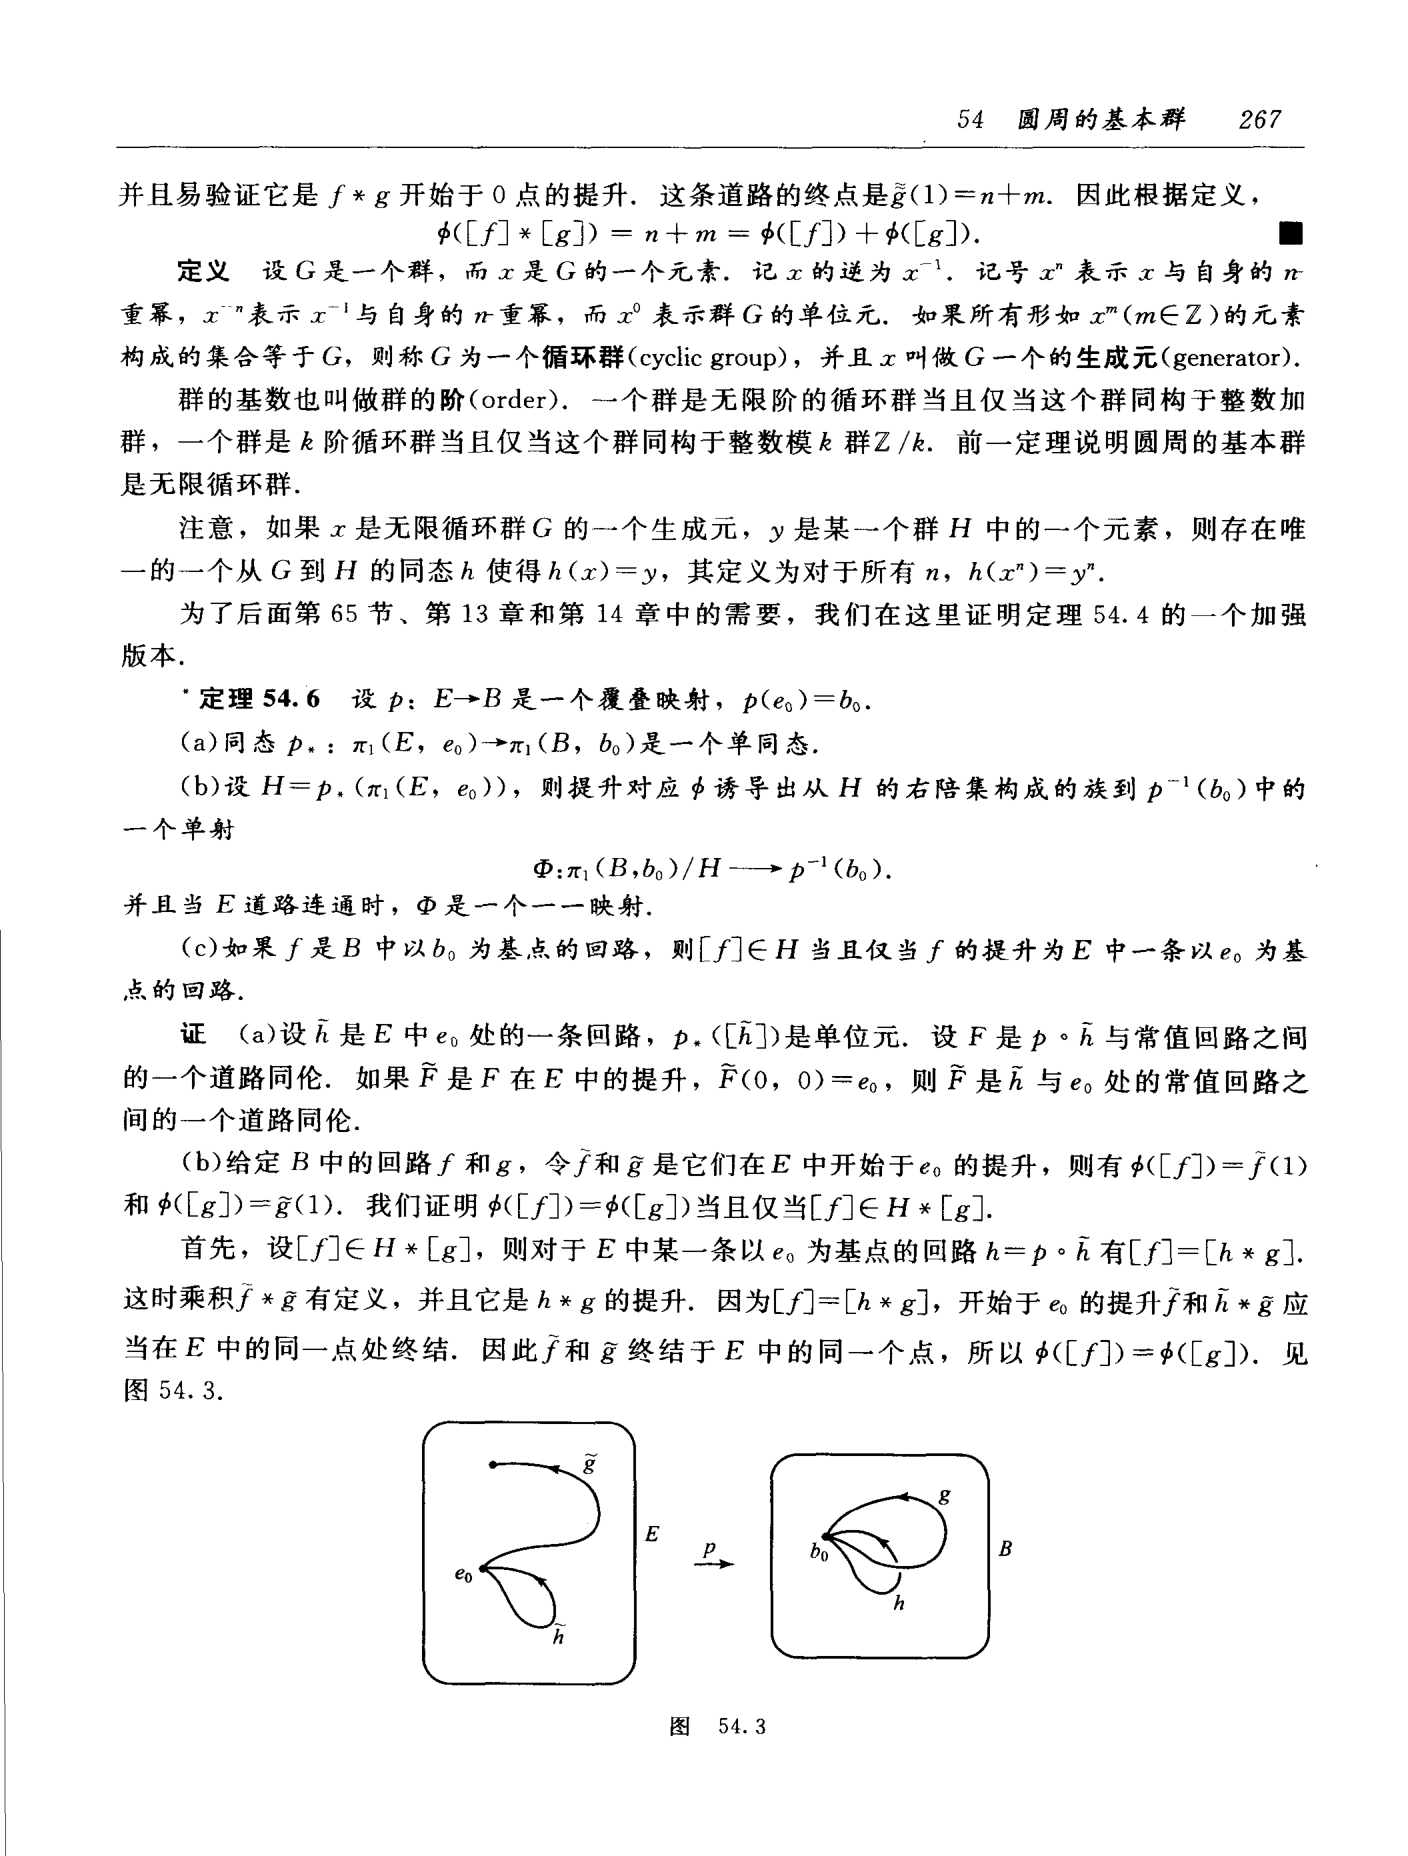
\includegraphics[width=0.6\textwidth]{image/fig-54-3.png}
\caption{定理 \cref{theorem:ch09-sec54-54-6} 的证明.}
\label{figure:ch09-fig-54-3}
\end{figure}

\begin{definition}[循环群]
\label{definition:ch09-sec54-cyclic}
设 $G$ 是一个群, 而 $x$ 是 $G$ 的一个元素. 记 $x$ 的逆为 $x^{-1}$. 记号 $x^n$ 表示 $x$ 与自身的 $n$ 重幂, $x^{-n}$ 表示 $x^{-1}$ 与自身的 $n$ 重幂, 而 $x^0$ 表示群 $G$ 的单位元. 如果所有形如 $x^m$ ($m\in\mathbb{Z}$) 的元素构成的集合等于 $G$, 则称 $G$ 为一个\textbf{循环群}(cyclic group), 并且 $x$ 叫做 $G$ 一个\textbf{生成元}(generator).
\end{definition}

群的基数也叫做群的\textbf{阶}(order). 一个群是无限阶的循环群当且仅当这个群同构于整数加群, 一个群是 $k$ 阶循环群当且仅当这个群同构于整数模 $k$ 群 $\mathbb{Z}/k$. 前一定理说明圆周的基本群是无限循环群.

注意, 如果 $x$ 是无限循环群 $G$ 的一个生成元, $y$ 是某一个群 $H$ 中的一个元素, 则存在唯一的一个从 $G$ 到 $H$ 的同态 $h$ 使得 $h(x)=y$, 其定义为对于所有 $n$, $h(x^n)=y^n$.

为了后面第 65 节、第 13 章和第 14 章中的需要, 我们在这里证明定理 \cref{theorem:ch09-sec54-54-4} 的一个加强版本.

\begin{theorem}
\label{theorem:ch09-sec54-54-6}
设 $p\colon E\to B$ 是一个覆叠映射, $p(e_0)=b_0$.
\begin{enumerate}
\item 同态 $p_*\colon\pi_1(E,e_0)\to\pi_1(B,b_0)$ 是一个单同态.
\item 设 $H=p_*(\pi_1(E,e_0))$, 则提升对应 $\phi$ 诱导出从 $H$ 的右陪集构成的族到 $p^{-1}(b_0)$ 中的一个单射
\[
\Phi\colon\pi_{1}(B,b_{0})/H\longrightarrow p^{-1}(b_{0}).
\]
并且当 $E$ 道路连通时, $\Phi$ 是一个一一映射.
\item 如果 $f$ 是 $B$ 中以 $b_0$ 为基点的回路, 则 $[f]\in H$ 当且仅当 $f$ 的提升为 $E$ 中一条以 $e_0$ 为基点的回路.
\end{enumerate}
\end{theorem}


\begin{proof}
(a) 设 $\tilde{h}$ 是 $E$ 中 $e_0$ 处的一条回路, $p_*([\tilde{h}])$ 是单位元. 设 $F$ 是 $p\circ\tilde{h}$ 与常值回路之间的一个道路同伦. 如果 $\widetilde{F}$ 是 $F$ 在 $E$ 中的提升, $\widetilde{F}(0,0)=e_0$, 则 $\widetilde{F}$ 是 $\tilde{h}$ 与 $e_0$ 处的常值回路之间的一个道路同伦.

(b) 给定 $B$ 中的回路 $f$ 和 $g$, 令 $\tilde{f}$ 和 $\tilde{g}$ 是它们在 $E$ 中开始于 $e_0$ 的提升, 则有 $\phi([f])=\tilde{f}(1)$ 和 $\phi([g])=\tilde{g}(1)$. 我们证明 $\phi([f])=\phi([g])$ 当且仅当 $[f]\in H*[g]$.

首先, 设 $[f]\in H*[g]$, 则对于 $E$ 中某一条以 $e_0$ 为基点的回路 $h=p\circ\tilde{h}$ 有 $[f]=[h*g]$. 这时乘积 $\tilde{f}*\tilde{g}$ 有定义, 并且它是 $h*g$ 的提升. 因为 $[f]=[h*g]$, 开始于 $e_0$ 的提升 $\tilde{f}$ 和 $\tilde{h}*\tilde{g}$ 应当在 $E$ 中的同一点处终结. 因此 $\tilde{f}$ 和 $\tilde{g}$ 终结于 $E$ 中的同一个点, 所以 $\phi([f])=\phi([g])$. 见图 \cref{figure:ch09-fig-54-3}.

\end{proof}

\subsection*{习题}

\begin{exercise}
设空间 $Y$ 的拓扑是离散的. 证明: 如果 $p\colon X\times Y\to X$ 是对于第一个坐标的投射, 则 $p$ 是一个覆叠映射.
\end{exercise}

\begin{exercise}
设 $p\colon E\to B$ 是连续的满射, 又设 $U$ 是 $B$ 的一个被 $p$ 均衡地覆盖着的开集. 证明: 如果 $U$ 是连通的, 则 $p^{-1}(U)$ 的片状分拆是唯一的.
\end{exercise}

\begin{exercise}
设 $p\colon E\to B$ 是覆叠映射, 又设 $B$ 是连通的. 证明: 如果对于某一个 $b_0\in B$, $p^{-1}(b_0)$ 恰有 $k$ 个元素, 则对于每一个 $b\in B$, $p^{-1}(b)$ 也恰有 $k$ 个元素. 在这种情形下, $E$ 称为 $B$ 的 $k$-\textbf{重覆叠}($k$-fold covering).
\end{exercise}

\begin{exercise}
设 $q\colon X\to Y$ 和 $r\colon Y\to Z$ 都是覆叠映射, 令 $p=r\circ q$. 证明: 如果对于每一个 $z\in Z$, $r^{-1}(z)$ 是有限的, 则 $p$ 是一个覆叠映射.
\end{exercise}

\begin{exercise}
证明例 \cref{example:ch09-sec53-3} 中的映射是覆叠映射. 将这个映射推广为 $p(z)=z^n$.
\end{exercise}

\begin{exercise}
设 $p\colon E\to B$ 是覆叠映射.
\begin{enumerate}
\item 如果 $B$ 是 Hausdorff、正则、完全正则或者局部紧致的 Hausdorff 空间, 则 $E$ 满足同样的拓扑性质. [提示: 如果 $\{V_\alpha\}$ 是 $p^{-1}(U)$ 的一个片状分拆, $C$ 是 $B$ 的一个闭子集, 它包含于 $U$, 则 $p^{-1}(C)\cap V_\alpha$ 是 $E$ 的一个闭子集.]
\item 如果 $B$ 是紧致的并且对于每一个 $b\in B$, $p^{-1}(b)$ 是有限的, 则 $E$ 也是紧致的.
\end{enumerate}
\end{exercise}
